\documentclass{standalone}
\usepackage{tikz}
\begin{document}
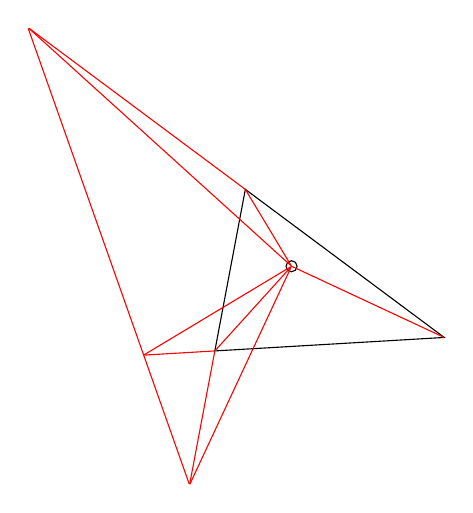
\begin{tikzpicture}[x=1pt,y=1pt]
\draw[red] (122.48,-190.54) -- (131.51,-142.72);
\draw[red] (131.37,-142.46) -- (106.09,-143.95);
\draw[red] (64.39,-25.84) -- (142.45,-83.97);
\draw (142.58,-84.06) -- (214.46,-137.58) -- (131.56,-142.45) -- cycle;
\draw (159.28,-111.85) circle (2.00);
\draw[red] (142.58,-84.06) -- (159.28,-111.85);
\draw[red] (131.56,-142.45) -- (159.28,-111.85);
\draw[red] (214.46,-137.58) -- (159.28,-111.85);
\draw[red] (159.05,-112.33) -- (122.52,-190.64);
\draw[red] (158.98,-111.57) -- (64.40,-25.91);
\draw[red] (106.02,-143.85) -- (158.94,-112.05);
\draw[red] (64.13,-25.91) -- (122.28,-190.46);
\end{tikzpicture}
\end{document}
